\documentclass[prb,aps,twocolumn,floatfix,amsmath,amssymb,superscriptaddress,tightenlines]{revtex4}
\usepackage{graphicx}
\usepackage{epstopdf}
\usepackage{amsfonts}
\usepackage{bm}
\usepackage{color}
\usepackage{ulem}
\begin{document}

\date{\today}
\title{Loop-Ratio VB QMC}


\author{Author}
\affiliation{Affiliation} 

\begin{abstract} 


Abstract

\end{abstract}
\maketitle

\section{Loop algorithm with ratio weighting}

We present an improvement on the recent algorithm using loop updates with quantum Monte Carlo in the valence bond basis, which is aids in the measurement of the Renyi entanglement entropies.

The {\bf ?topology?} of the loop-operator list is modified.

Differences:  links are changed across boundary between system copies, measurements values must be multiplied by $\langle Swap_x \rangle$ to get the value unmodified by the weight.

\subsection{Pre-initialization? Set-up? }
 
\subsubsection{Lattice}
%Possible types of lattices (bipartite, non-frustrated, BCs don't matter, interactions only btwn the two different sublattices)... nothing with the sign problem\\
	
%How many copies of the system?\\
The standard loop algorithm simulation contains two independent copies of the system to be studied, amounting to one VB-spin-operator list. 
%(they're not *really* independent.. they're connected by the loop-operator list.)
To measure $S_2$ an additional VB-spin-operator list is required, amounting to four copies of the original system.
In general we will have $2\alpha$ copies of the system, resulting in $\alpha$ VB-spin-operator structures.
	
We mush choose and initial VB state for each copy of the system (not necessarily all different) with bonds only between different sublattices. 
%(reference? or explain sublattices? don't want to introduce sublattice A \& B notation as it'll be confused with region A \& B.)
For each of these initial VB states a compatible initial spin state must also be chosen such that each valence bond has one site with spin up $\uparrow$ and the other with spin down $\downarrow$.

It is simplest to begin with the same spin states for both initial states within a single VB-spin-operator list, though the VB states on either side may be different.	
	
	
\subsubsection{Bond Operators}

Valence bond quantum Monte Carlo simulations are a type of ground state projection technique, and as such, we must decide how many times to apply the Hamiltonian to our trial state(s) in each step.  
This value $m$ is a convergence parameter for the simulation.
{\bf ((Something about the balance between large and small m.. need convergence.. don't want to waste simulations time.  Doesn't scale properly per site...   (((seems like you need less than a number of operators per site... like the number of ops/site that works for small systems is more than enough for large systems.. PLOTS)))   )) }


There are two types of bond operators, diagonal operators $H_{ab}(1)$ and off-diagonal operators $H_{ab}(2)$, which act of interacting pairs of sites (labelled $a$ and $b$ here)
\begin{eqnarray}
	H_{ab}(1) &=&(\tfrac{1}{4} - S^z_aS^z_b) \\
	H_{ab}(2) &=& -(S_a^xS_b^x + S_a^yS_b^y). 
		      %  = -\tfrac{1}{2}(S_a^+S_b^- + S_a^-S_b^+)
\end{eqnarray}
%where $S^x_i$, $S^y_i$, $S^z_i$ are the quantum spin operators acting on the $i^{\rm th}$ site.

Bond operators are chosen such that they only act on sites with antiparallel spins. 

\noindent
{\bf- parallel and antiparallel bond ops... the formulas and stuff

\noindent
- talk about convergence in the number of bond operators (plot prolly, eh?)\\
}

\subsection{Main Program}
\subsubsection{Building the loops}

\begin{figure} {
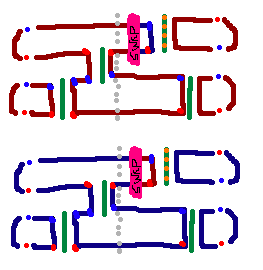
\includegraphics[width=2.4 in]{oplist.png} \caption{ 
\label{oplist} A possible VB-spin-operator diagram for a 4-site system with m=2 operators per copy of the system, {\bf (something about ratio and used to calculate the 2nd renyi entropy)
(also, make sure the two copies have *different* operators and loops, but still compatible spin configurations)}
}
} \end{figure}


\subsubsection{Flip...?}
\noindent 
{\bf
- keep the loops the same, flip all the spins.\\
- causes some diagonal operators to become off-diagonal and vice versa
}
\subsubsection{$\langle Swap_A \rangle$ measurement}
\noindent
{\bf 
- renyi measurement \\
- need to multiply by weight factor to get the actual measurement values\\
- energy (and other measurements) could be doubled (or alpha-ed) because we have multiple copies of the system
}
\subsubsection{Updating the operator list}
\noindent
{\bf- keep off-diagonal bond operators, move diagonal bond operators to a random, compatible spot.}
	
\subsection{Swap operator for $\alpha > 2$}

\begin{figure} {
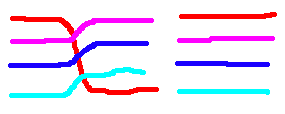
\includegraphics[width=2.4 in]{swap.png} \caption{ 
\label{swap_4} 
The cyclical permutation of states in region $A$ for four copies of a system.
}
} \end{figure}

\bibliography{}

\end{document}
